\chapter{Background}\chlabel{background}
%\pagenumbering{arabic}
%\section{Preliminaries}

%In this section, we give the preliminary results and concepts which
%are necessary for the understanding and development of the work in
%this thesis. We also establish notation and conventions used
%throughout. %Due to the elementary nature of our work, we  probability theory.

As before, we will agree that the base of logarithms in $\log x$ is
$2$.

%Since we are overwhelmingly concerned with binary encodings, we will
%agree now that base of logarithms in $\log x$ is $2$.
%That being said,
%some of the concepts presented further in this work need not strictly
%be restricted to the binary setting.

Due to the elementary nature of our work, we avoid the presentation of
probability theory. For a rigorous introduction to the basics of
probability theory, including Kolmogorov's axioms for probability
measures, and the study of random variables and their distributions,
see the book by Rohatgi and Saleh~\cite{rohatgi:probability}. We
similarly avoid a discussion of basic graph theory; the book by West
serves as a suitable introduction~\cite{west:graphtheory}.

%We will say that a sequence of random variables
%$X_1, X_2, \ldots, X_n$ is \emph{iid} if all random variables in the
%sequence are independent and identically distributed. If
%$X_1, X_2, \ldots, X_n$ is iid and uniformly distributed, we will say
%that it is \emph{iud}.
For a random variable $X : \Omega \to \R$ with probability density
$p : \Omega \to [0, 1]$, we will denote the probability of
$x \in \Omega$ as $p_x$. Finally, we will often refer to the following
result as the \emph{union bound}.
\begin{lem}[Boole's Inequality]
  For any sequence of events $A_1, A_2, \ldots$,
  \[
  \Pr\left[\bigcup_{i \geq 1} A_i\right] \leq \sum_{i \geq 1}
  \Pr[A_i].
  \]
\end{lem}

%A \emph{random variable} will be a function $X: S \to \R$, where $S$
%is a finite set. Each random variable determines a probability
%distribution such that:
%\[\Pr[X = x] = \frac{|X^{-1}(x)|}{|S|}\]
%A \emph{Bernoulli} random variable with parameter $p$, denoted
%$\text{Bernoulli}(p)$, will be a random variable $B : S \to \{0, 1\}$,
%where:
%\[\Pr[B = 1] = p \quad \text{and} \quad \Pr[B = 0] = 1 - p\]
%We will say that a sequence of random variables
%$X_1, X_2, \ldots, X_n$ which are independent
%Talk about notation. Base of logarithms, etc. Lambert W function.
%Maybe some stuff about probability. Probably not too important. Talk
%about iid and iud.

%The following classic result also becomes important.
%\begin{lem}[Jensen's Inequality]\lemlabel{jensen}
%  Let $f$ be a convex function and $X$ be a random variable. Then:
%  \[f(\E[X]) \leq \E[f(X)]\]
%
%  The inequality is reversed if $f$ is concave.
%\end{lem}

%\begin{lem}[Gibbs' Inequality]\lemlabel{gibbs}
%  If $\{p_1, \ldots, p_n\}$ and $\{q_1, \ldots, q_n\}$ are two
%  probability distributions, then:
%  \[\sum_{i = 1}^n p_i \log (1/p_i) \leq \sum_{i = 1}^n p_i \log (1/q_i)\]
%
%  with equality if and only if $p_i = q_i$ for all $1 \leq i \leq n$.
%\end{lem}
%\begin{proof}
%  USING JENSEN.
%\end{proof}
%\begin{thm}[Stirling's
%  Approximation~\cite{robbins:stirling}]\thmlabel{stirling}
%  \[n! = \sqrt{2 \pi n} \left(\frac{n}{e}\right)^n e^{r(n)},\]
%  where $r(n)$ satisfies $\frac{1}{12n + 1} < r(n) < \frac{1}{12n}$.
%\end{thm}

%\begin{lem}[Jensen's Inequality]\lemlabel{jensen}
%  If $f$ is a convex function and $X$ is a random variable, then
%  \[f(\E[X]) \leq \E[f(X)].\]
%  The inequality is reversed if $f$ is concave.
%\end{lem}

\section{Prefix-Free Codes}

\begin{defn}
  For a set $\Sigma$, the set $\Sigma^*$ is defined to be the set of
  all finite length strings with characters in $\Sigma$, including the
  empty string $\epsilon$.
\end{defn}
For example,
$\{0, 1\}^* = \{\epsilon, 0, 1, 00, 01, 10, 11, \ldots\}$, the set of
finite length binary bit strings.

\begin{defn}
  A \emph{code} for the set $\Omega$ is an injective function
  $C : \Omega \to \{0, 1\}^*$. We say that $\Omega$ is \emph{encoded},
  and that the values of $C$ are \emph{codewords}.
\end{defn}

The length of the codeword $x \in \Omega$ will be denoted by $|C(x)|$.

\begin{defn}
  A string $x$ is a \emph{prefix} of the string $y$ if there exists
  some string $z$ such that $xz = y$.
\end{defn}

\begin{defn}
  A code $C : \Omega \to \{0, 1\}^*$ is \emph{prefix-free} if, for any
  $x, y \in \Omega$, $C(x)$ is not a prefix of $C(y)$.
\end{defn}

Note that $\epsilon$ can never be a codeword in a prefix-free code.

\begin{defn}
  A \emph{partial prefix-free code} is a function $C : \Omega \to \{0,
  1\}^* \cup \{\bot\}$ which is a prefix-free code on the set $\{x :
  C(x) \neq \bot\}$, called its \emph{domain}. We will say that $C(x)
  = \bot$ is undefined, and formally $|\bot| = \infty$.
\end{defn}

A partial prefix-free code $C$ is vacuously bijective on its domain,
and for all intents and purposes is bijective on the set $\Omega$, in
the sense that we are not concerned with undefined codewords.

We can also consider \emph{uniquely decipherable codes}: a code ${C :
  \Omega \to \{0, 1\}^*}$ is uniquely decipherable if for any $x_1,
\dots, x_n \in \Omega$, the string $C(x_1) \cdots C(x_n)$ can only be
written one way as a concatenation of codewords. These are the codes
for which there exists an effective decoding procedure. Prefix-free
codes are sometimes called instantaneous codes, since any string of
codewords from a prefix-free code can be read from left to right and
decoded as soon as each codeword is recognized. In fact, uniquely
decipherable codes are a strict generalization of prefix-free
codes. However, perhaps surprisingly, we will see that prefix-free
codes suffice for our purposes.

\begin{figure}
  \centering
  \includegraphics{bintree}
  \caption{A prefix-free code $C$ for the set $\{a, b, c, d, e, f\}$
    with its corresponding binary tree.}
  \figlabel{bintree}
\end{figure}

It is helpful to think of a partial prefix-free code $C$ as a (rooted
ordered) binary tree whose leaf set is the domain of $C$, as in
\figref{bintree}. In fact, there is a correspondence between rooted
ordered binary trees and prefix-free codes. The code for an element
$x \in \Omega$ in such a tree is described by the sequence of turns in
its root-to-leaf path in this tree, where a left turn (respectively, a
right turn) corresponds to a zero bit (respectively, a one
bit). Conversely, a prefix-free code describes a binary tree
recursively, where each codeword beginning with a zero bit
(respectively, a one bit) is given to the root's left subtree
(respectively, right subtree).

\begin{figure}
  \centering
  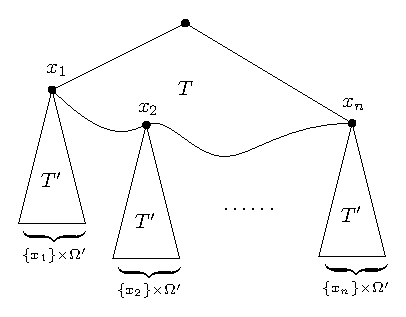
\includegraphics{prefixcodecomposition}
  \caption{The composition of prefix-free codes is prefix-free.}
  \figlabel{prefixcodecomposition}
\end{figure}

Let $C : \Omega \to \{0, 1\}^*$ and $C' : \Omega' \to \{0, 1\}^*$ be
prefix-free codes corresponding to trees $T$ and $T'$. Consider the
code $C \cdot C' : \Omega \times \Omega' \to \{0, 1\}^*$, where
\[
(C \cdot C')(x, y) = C(x) C'(y).
\]
It is easily seen that the tree of \figref{prefixcodecomposition}, in
which each leaf of $T$ is replaced by a copy of $T'$, is the tree
corresponding to $C \cdot C'$. In other words, the composition of
prefix-free codes is prefix-free. We will make use of this fact.

Let $h$ be such that $2^{h - 1} < |\Omega| \leq 2^{h}$, and consider
the complete binary tree of height $h$. If we assign the leftmost
leaves of this tree to the elements of $\Omega$ and discard the
remaining leaves, truncating the tree, we effectively obtain a
prefix-free code $C$ for $\Omega$ for which
\begin{align}
  |C(x)| = h = \ceil{\log |\Omega|}, \eqlabel{fixed-length}
\end{align}
\emph{i.e.}~any finite set $\Omega$ can be given a prefix-free code
for which every codeword has length $\ceil{\log |\Omega|}$. We will
call this the \emph{fixed-length encoding} of $\Omega$. It is
important to note that such a code requires the decoder to know the
size of $\Omega$ to determine the string's delimitations.

\begin{exm}
  In some cases, we are interested in encoding a set of size
  $n!$. Recall Stirling's approximation,
  \[
  n! = \sqrt{2 \pi n} \left(\frac{n}{e}\right)^n e^{r(n)},
  \]
  where $r(n)$ satisfies
  $\frac{1}{12n + 1} < r(n) < \frac{1}{12n}$~\cite{robbins:stirling}.
  We can use this approximation to bound the length of fixed-length
  codes of these sets, so
  \begin{align}
    \log n! & = n \log n - n \log e + \frac{1}{2} \log n + \log \sqrt{2\pi} + \varTheta(1/n)  \notag \\
            & \leq n \log n - n \log e + O(\log n). \eqlabel{perm-code-loose} \enspace
  \end{align}

  Note that such a fixed-length code would have length
  $\ceil{\log n!}$, but we have chosen to ignore the ceiling in this
  analysis for reasons to be made clear later.
\end{exm}

The correspondence between prefix-free codes and binary trees is
useful in proving the next result, which is central to the function of
prefix-free encoding arguments.
\begin{defn}
  A function $\ell : \Omega \to \R$ is said to \emph{satisfy Kraft's
    condition} if
  \[\sum_{x \in \Omega} 2^{-\ell(x)} \leq 1.\]
\end{defn}

\begin{lem}[Kraft's Inequality~\cite{kraft:inequality}]\lemlabel{kraft-inequality}
  If $C : \Omega \to \{0, 1\}^*$ is a prefix-free code, then
  $|C(\cdot)| : \Omega \to \N$ satisfies Kraft's
  condition. Conversely, given some function $\ell : \Omega \to \N$
  satisfying Kraft's condition, there exists a prefix-free code
  $C : \Omega \to \{0, 1\}^*$ for which $|C(x)| = \ell(x)$ for all
  $x \in \Omega$.
\end{lem}
\begin{proof}
  First, consider the tree corresponding to the prefix-free code
  $C$. Let each degree 2 node represent a $\text{Bernoulli}(1/2)$
  random variable, where each one of the left or right children is
  chosen with probability $1/2$; degree 1 nodes automatically choose
  their only child. Let $X$ denote the leaf node obtained by following
  this random process from the root. Then
  \[1 = \Pr\left[\bigcup_{x \in \Omega} (X = x)\right] = \sum_{x \in \Omega} \Pr[X =
  x] \geq \sum_{x \in \Omega} 2^{-|C(x)|},\]
  with equality if and only if each internal node has degree 2.

  Conversely, write $\ell(x_1) \leq \cdots \leq \ell(x_n)$. Consider
  the complete binary tree $T$ of height $\ell(x_n)$. We transform $T$
  into a tree which corresponds to a prefix-free code satisfying
  Kraft's condition.

  Choose a node $u_1$ at depth $\ell(x_1)$ (say, the first encountered
  in a depth first traversal) and remove its subtree from $T$. The
  code $C(x_1)$ will correspond to the root-to-leaf path to
  $u_1$. Continue this process for depths $\ell(x_2)$ through
  $\ell(x_n)$. The only way this process can fail is if the tree has
  no leaves at depth $\ell(x_n)$ at any point. But the number of
  leaves at depth $\ell(x_n)$ before step $j$ in which the code
  $C(x_j)$ is assigned is
  \begin{align*}
    2^{\ell(x_n)} - \sum_{i = 1}^{j - 1} 2^{\ell(x_n) - \ell(x_i)} =
    2^{\ell(x_n)}\left(1 - \sum_{i = 1}^{j - 1} 2^{-\ell(x_i)}\right)
    > 2^{\ell(x_n)}\left(1 - \sum_{i = 1}^n 2^{-\ell(x_i)}\right)
    \geq 0,
  \end{align*}
  so the process completes. If $T$ has any extra leaves which do not
  correspond to elements of $\Omega$, then prune them from the
  tree. The remaining tree $T$ corresponds to a prefix-free code $C$
  for which $|C(x_i)| = \ell(x_i)$ for each $i$.
\end{proof}

It is a fact that \lemref{kraft-inequality} also holds for uniquely
decipherable codes. Therefore, in some sense, we are justified in
restricting our study strictly to prefix-free codes, since for any
uniquely decipherable encoding of a set, there exists a prefix-free
code for the same set with exactly the same codeword
lengths~\cite{gallager:informationtheory,
  mcmillan:uniquedecipherability}.

Suppose now that we are interested in encoding an incremental sequence
of choices for which the number of options at any point depends upon
previous choices. Indeed, we define sets $\Omega_1, \ldots, \Omega_t$
such that $\Omega_1$ is fixed and $\Omega_{i + 1}$ depends on some
sequence of selections $(x_1, \ldots, x_i) \in \Omega_1 \times \cdots
\times \Omega_i$. The set $\Omega_1 \times \cdots \times \Omega_t$ is
called the \emph{decision space} for the sequence of choices $x =
(x_1, \ldots, x_t)$. Suppose that the decision space for $x$ has size
$d$. We can encode $x$ by presenting a sequence of fixed-length
encodings for $x_i \in \Omega_i$, and the code for $x$ then has length
\[
\sum_{i = 1}^t \ceil{\log |\Omega_i|} \leq \log \prod_{i=1}^t
|\Omega_i| + t = \log d + t,
\]
and indeed, each choice may incur an extra bit in the code,
\emph{e.g.}~if $|\Omega_i| = 2^{n} + 1$, then this code has length $nt + t$, but
\[
\log d = \log (2^n + 1)^t = t \log (2^n + 1) \leq nt + O(t 2^{-n}).
\]

The next result, attributed to Jiang, allows us to encode $x$ without
requiring extra bits.
\begin{lem}[Lucier \emph{et al.}~\cite{lucier.jiang.li:quicksort}]\lemlabel{incremental-code}
  If $x$ is an incremental choice of values with a decision space of
  size $d$, then $x$ can be encoded with $\ceil{\log d}$ bits.
\end{lem}
\begin{proof}
  Suppose that $x = (x_1, \ldots, x_t)$ has the decision space
  $\Omega_1 \times \cdots \times \Omega_t$, and let
  $k_i \in \{0, \ldots, |\Omega_i| - 1\}$ be the index of $x_i$ in
  $\Omega_i$, for each $1 \leq i \leq t$. Consider the integer
  \[k = k_1 + k_2 |\Omega_1| + k_3 |\Omega_1| |\Omega_2| + \cdots +
  k_t \prod_{i=1}^{t-1}|\Omega_i|.\] We know that
  \[0 \leq k \leq (|\Omega_1| - 1) + (|\Omega_2| - 1)|\Omega_1| +
  \cdots + (|\Omega_t| - 1)\prod_{i = 1}^{t - 1} |\Omega_i| = d - 1,\]
  since telescoping kills each $\prod |\Omega_i|$ except for the last
  one. So our encoding for $x$ is simply a fixed-length encoding of
  $k$.

  To decode $x = (x_1, \ldots, x_t)$ from the value of $k$, we can
  compute and retrieve $k_1 = k \bmod |\Omega_1|$, since we know
  $|\Omega_1|$. From the value $k_1$, we determine $x_1$, which in
  turn determines $|\Omega_2|$. We can then retrieve $k_2$ from
  $k_2 |\Omega_1| + k_1 = k \bmod |\Omega_2|$, so we determine
  $x_2$. Continuing in this way, we can determine all of
  $x = (x_1, \ldots, x_t)$. From \eqref{fixed-length}, this code has
  length $\ceil{\log d}$.
\end{proof}

This result becomes useful when analyzing constant factors or lower
order terms, or if the number of choices is significant
(\emph{e.g.}~in \secref{records}). In many cases, only a constant
number of choices are made, which causes only at most an insignificant
constant number of wasted bits. Moreover, other approximations in
codeword lengths sometimes involve a super-constant lower order term,
in which case the result is likely useless (\emph{e.g.}~whenever
\eqref{perm-code-loose} is invoked).

\section{Entropy}

Each code $C : \Omega \to \{0, 1\}^*$ has an associated random
variable of codeword lengths $|C(\cdot)| : \Omega \to \N$, which is
our main object of study. The following definition will help to
understand and quantify codeword length optimality.
\begin{defn}
  The \emph{entropy} $\ent(X)$ of a random variable
  $X : \Omega \to \R$ with probability density $p$ is
  \[\ent(X) = \sum_{x \in \Omega} p_x \log \frac{1}{p_x},\]
  sometimes denoted by $\ent(p)$. The \emph{binary entropy function}
  $H : [0, 1] \to \R$ is defined by
  \[H(\alpha) = \ent(\text{Bernoulli}(\alpha)) = \alpha \log
  \frac{1}{\alpha} + (1 - \alpha) \log \frac{1}{1 - \alpha},\]
  where $H(0) = H(1) = 0$.
\end{defn}

In this thesis, we sometimes use the following approximation of the
binary entropy function:
\begin{align}
  H(\alpha) & = \alpha \log \frac{1}{\alpha} + (1 - \alpha) \log \frac{1}{1 - \alpha} \notag \\
  & = \alpha \log \frac{1}{\alpha} + (1 - \alpha) \log \left(1 + \frac{\alpha}{1 - \alpha}\right) \notag \\
  & \leq \alpha \log \frac{1}{\alpha} + \alpha \log e = \alpha \log
  (e/\alpha), \eqlabel{entropy-approx}
\end{align}
since $1 + x \leq e^x$ for every $x \in \R$. See
\figref{entropy-approx-plot} for a comparison between $H(\alpha)$ and
its approximation.

\begin{figure}
  \centering
  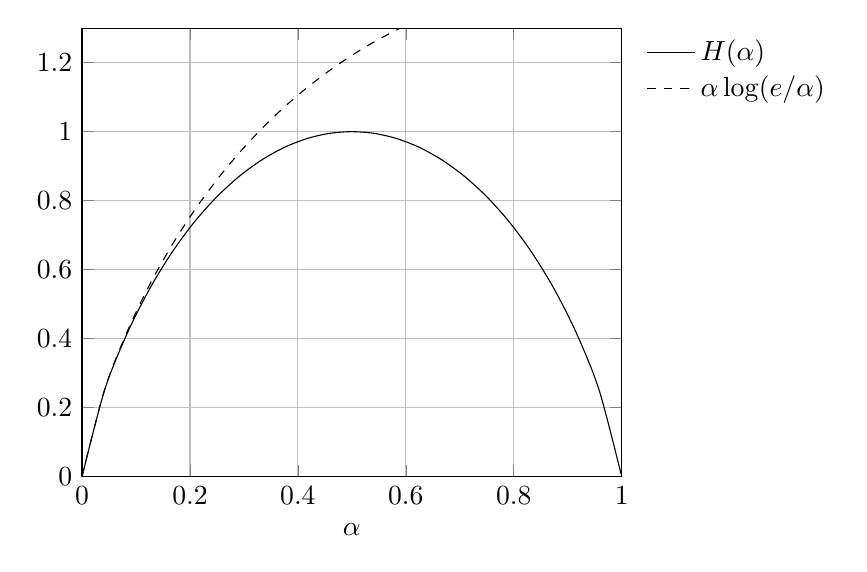
\begin{tikzpicture}
    \begin{axis}[
      xlabel=$\alpha$,
      legend cell align=left,
      legend pos=outer north east,
      legend style={draw=none},
      grid=major,
      ymin=0,
      ymax=1.3,
      xmin=0,
      xmax=1
      ]

      \addplot[
      smooth,
      domain=0:1
      %blue
      ]
      {-x*log2(x) - (1 - x)*log2(1 - x)};
      \addlegendentry{$H(\alpha)$}
    
      \addplot[
      smooth,
      domain=0:1,
      style=dashed
      %color=red
      ]
      {-x*log2(x) + x*log2(e)};
      \addlegendentry{$\alpha \log (e/\alpha)$}
    \end{axis}
  \end{tikzpicture}
  \caption{Comparison between $H(\alpha)$ and its approximation from
    \eqref{entropy-approx}.}
  \figlabel{entropy-approx-plot}
\end{figure}

We will see how the entropy of $X$ describes the expected amount of
information in bits required to represent $X$. Consider the following
examples:
\begin{exm}
  Let $X : \{1, \ldots, n\} \to \R$ be uniformly distributed. From
  \eqref{fixed-length}, we can encode each element of
  $\{1, \ldots, n\}$ with a fixed-length code of length
  $\ceil{\log n}$. Moreover, we easily see that $\ent(X) = \log n$.
\end{exm}

\begin{exm}
  Let $X : \{1, \ldots, n\} \to \R$ have probability density
  $p_i = 1/2^i$ for $1 \leq i < n$, and $p_n = 1/2^{n - 1}$. Then
  \[\lim_{n \to \infty} \ent(X) = 2.\]

  This is a dramatic difference in entropy from the previous example,
  demonstrating that a fixed-length code for $X$ would be terribly
  inefficient, since several elements of $X$ appear with exponentially
  low probability. In this case, a more judicious coding strategy is
  required. Consider the code $C$ such that
  \[
  C(i) = \left\{
  \begin{array}{ll}
    0^{i - 1} \; 1 & \mbox{if $1 \leq i < n$};\\
    0^{n - 1} & \mbox{if $i = n$}.
  \end{array} \right.
  \]
  Notice that this code is prefix-free with expected codeword length
  exactly $\ent(X)$.
\end{exm}

We can prove that $\log (1/p_x)$ is the optimal codeword length for
any element $x \in \Omega$. We rely on the following classic result.
\begin{thm}[Jensen's Inequality]\thmlabel{jensen}
  For any concave function $f$ and any random variable $X$,
  \[
  \E[f(X)] \leq f(\E[X]) .
  \]
  This inequality is reversed if $f$ is convex.
\end{thm}
\begin{thm}\thmlabel{optimal-kraft}
  If $\ell : \Omega \to \R$ satisfies Kraft's condition, where
  $\Omega$ is endowed with the probability density $p$, then
  \[
  \sum_{x \in \Omega} p_x \log (1/p_x) = \ent(p) \leq \E[\ell(x)] = \sum_{x \in \Omega} p_x \ell(x) .
  \]
\end{thm}
\begin{proof}
  We examine the value $\ent(p) - \E[\ell(x)]$, where
  \begin{align}
    \ent(p) - \E[\ell(x)] &= \sum_{x \in \Omega} p_x \log (1/p_x) - \sum_{x \in \Omega} p_x \ell(x) \notag \\
                          &= \sum_{x \in \Omega} p_x \log \left(\frac{2^{-\ell(x)}}{p_x}\right) \notag \\
                          &= \E\left[\,\log \left(\frac{2^{-\ell(x)}}{p_x}\right)\,\right] \notag \\
                          &\le \log \left(\E\left[\,\frac{2^{-\ell(x)}}{p_x}\,\right]\right), \eqlabel{entropy-optimal}
  \end{align}
  by Jensen's inequality, since $\log$ is a concave function. Then,
  \eqref{entropy-optimal} becomes
  \[
  \log \left(\E\left[\,\frac{2^{-\ell(x)}}{p_x}\,\right]\right) = \log
  \left( \sum_{x \in \Omega} 2^{-\ell(x)} \right) \le \log 1 = 0
  \]
  by \lemref{kraft-inequality}.
\end{proof}
Shannon proved the following result, which describes how entropy
relates to codeword lengths; in addition to satisfying the conditions
of the previous theorem, codeword lengths must also be integers.
\begin{thm}[Noiseless Coding Theorem~\cite{shannon:mathematical}]\thmlabel{noiseless-coding}
  If $C : \Omega \to \{0, 1\}^*$ is a prefix-free code with
  probability density $p$ minimizing its expected codeword length,
  then
  \[\ent(p) \leq \E\left[\,|C(x)|\,\right] < \ent(p) + 1.\]
\end{thm}

%In this sense, $\log (1/p_x)$ is the optimal codeword length for any
%element $x \in \Omega$, since
%$\E\left[\,|C(x)|\,\right] = \sum_{x \in \Omega} p_x |C(x)|$, and
%$\ent(p) = \sum_{x \in \Omega} p_x \log (1/p_x)$. In fact, it can be
%shown through standard optimization techniques that for any
%(potentially non-integer valued) function $\ell : \Omega \to \R$
%satisfying Kraft's condition and any probability density
%$p : \Omega \to [0, 1]$, the minimum value of
%$\sum_{x \in \Omega} p_x \ell(x)$ is attained when
%$\ell(x) = \log (1/p_x)$, so that
%\[\sum_{x \in \Omega} p_x \ell(x) = \ent(p).\]

\section{Shannon-Fano Codes}

Earlier, we showed how to encode the set $\Omega$ using a fixed-length
code. Suppose now that $\Omega$ is augmented with a probability
distribution. Our goal is to provide a better code, in the sense that
more probable elements are given appropriately shorter codes.

The \emph{Shannon-Fano code} for $\Omega$ is a prefix-free code
constructed from a probability distribution over the elements of
$\Omega$~\cite{fano:transmission, shannon:mathematical}.

%More specifically, the algorithm constructs a
%full binary tree with the elements of $X$ as its leaves, and the
%encoding is understood from this tree.

Let $\Omega$ be endowed with the probability density $p$. Since
\[\sum_{x \in \Omega} 2^{-\ceil{\log (1/p_x)}} \leq \sum_{x \in \Omega} 2^{-\log
  (1/p_x)} = \sum_{x \in \Omega} p_x = 1,\]
then the proof of \lemref{kraft-inequality} gives a deterministic
construction for a prefix-free code $C : \Omega \to \{0, 1\}^*$, where
\[
|C(x)| = \Ceil{\log \frac{1}{p_x}}. \eqlabel{shannon-fano-optimality}
\]
This is the Shannon-Fano code: see \figref{shannon-fano} for an
example construction.

%This specific code is the Shannon-Fano
%code.
%
%The Shannon-Fano code $C(x_i)$ for
%$x_i$ will be shown to have length:
%\[|C(x_i)| = \ceil{\log (1/p_{x_i})}\]
%
%Indeed, by \lemref{kraft-inequality}:
%\[\sum_{x \in X} 2^{-|C(x)|} \leq \sum_{x \in X} 2^{-\log (1/p_x)} =
%\sum_{x \in X} p_x = 1\]
%
%so a prefix-free code with such codeword lengths does exist, and it is
%described by the construction given in the proof of
%\lemref{kraft-inequality}.

\begin{figure}
  \centering
  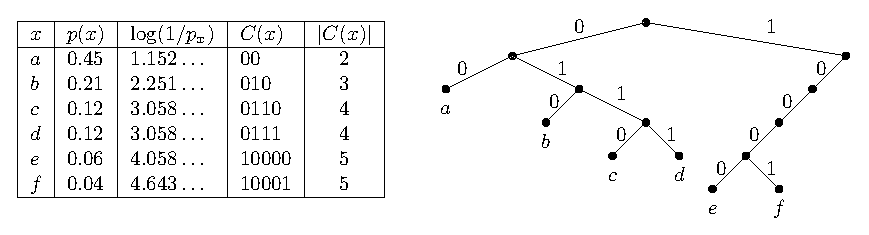
\includegraphics{shannon-fano}
  \caption{The Shannon-Fano code and corresponding tree for a set and
    probability distribution as given by the construction in
    \lemref{kraft-inequality}. Notice the values $\log (1/p_x)$ and
    $|C(x)|$.}
  \figlabel{shannon-fano}
\end{figure}

A useful fact about the codes presented in this section is that they
are locally optimal in the sense of \thmref{noiseless-coding}, since
the optimal codeword length for $x \in \Omega$ is $\log (1/p_x)$.
Local optimality will prove to be more useful to us than global
optimality.

Note that if we choose $p$ to be the uniform distribution, then
$p_x = 1/|\Omega|$, and the Shannon-Fano code $C$ for $\Omega$ is such
that
\[
|C(x)| = \ceil{\log |\Omega|},
\]
as seen previously with \eqref{fixed-length}.

We will mostly apply Shannon-Fano codes in the encoding of random bit
strings $x = x_1 \cdots x_n$, where all $x_i$ are independent and
identically distributed as $\text{Bernoulli}(p)$ random variables. We
will say that $p$ is the \emph{parameter} for this Shannon-Fano
code. Let $n_1(x)$ denote the number of one bits in $x$, and $n_0(x) =
n - n_1(x)$ denote the number of zero bits in $x$. Then, a particular
string $x$ appears with probability exactly $p^{n_1(x)} (1 -
p)^{n_0(x)}$. In this case, the codeword for $x$ has length
\[|C(x)| = \left\lceil n_1(x) \log \frac{1}{p} + n_0(x) \log
  \frac{1}{1 - p} \right\rceil.\]

\begin{exm}
  We are often concerned with producing fixed-length encodings for
  sets of size ${n \choose k}$. Since
  \[
  \left(\frac{k}{n}\right)^k \left(1 - \frac{k}{n}\right)^{n - k} =
  2^{-n H(k/n)}
  \]
  is the probability that a particular $n$-bit binary string with
  exactly $k$ ones appears if each bit is chosen with probability
  $k/n$, then the Shannon-Fano code with parameter $k/n$ for this bit
  string has length $\lceil n H(k/n) \rceil$. Since the number of bit
  strings of length $n$ containing exactly $k$ ones is $\binom{n}{k}$,
  then
  \[
  \log \binom{n}{k} \leq \lceil n H(k/n) \rceil,
  \]
  establishing a bound on the length of fixed-length encodings for
  such sets---in fact, using \thmref{optimal-kraft} we can show that
  this ceiling can be omitted, and
  \begin{align}
    \log \binom{n}{k} \leq n H(k/n). \eqlabel{binom-code-tight}
  \end{align}
  %Again, from
  %\thmref{stirling} and \eqref{perm-code-tight} we see that
  %\begin{align}
  %  \log {n \choose k} & = \log n! - \log k! - \log (n - k)! \notag \\
  %                     & = n \log n - k \log k - (n - k) \log (n - k) + \frac{1}{2} \log \frac{n}{k(n - k)} + \varTheta(1/k) \notag \\
  %                     & \leq k(\log n - \log k) + (n - k) (\log n - \log (n - k)) + O(1) \notag \\
  %                     & = n H(k/n) + O(1).  \eqlabel{binom-code-tight}
  %\end{align}
  Applying the estimate from \eqref{entropy-approx}, we obtain that
  \begin{align}
    \log {n \choose k} \leq k \log n - k \log k + k \log e. \eqlabel{binom-code-loose}
  \end{align}
  This estimate is only useful when $k/n$ is small.  We can instead
  obtain a similar and slightly worse bound than
  \eqref{binom-code-tight} by relying on Stirling's approximation and
  the fact that $\binom{n}{k} = \frac{n!}{k!(n - k)!}$.
\end{exm}

We give an example of when it might be more useful to apply
\eqref{binom-code-tight} over \eqref{binom-code-loose}: suppose we
wish to encode a sparse bit string, \emph{i.e.}~a bit string in which
$n_1(x)$ is relatively small.
\begin{lem}\lemlabel{bitstring-compression}
  Let $x \in \{0, 1\}^n$, where $n_1(x) \leq \alpha n$ for some
  $0 \leq \alpha \leq 1/2$. Then, we can give a prefix-free code for
  $x$ of length at most $\log n + n H(\alpha) + O(1)$.
\end{lem}
\begin{proof}
  Encode $x$ by giving the value $n_1(x)$, and then the set of
  positions of the $n_1(x)$ ones in the string. This allows us to
  deduce the entire bit string. Since $n_1(x) \leq \alpha n$ and
  $0 \leq \alpha \leq 1/2$, then
  ${n \choose n_1(x)} \leq {n \choose \alpha n}$, so our code has
  length at most
  \[\log n + n H(\alpha) + O(1). \qedhere\]
\end{proof}

In this case, \eqref{binom-code-tight} grants us immediate higher
order savings for any $0 \leq \alpha < 1/2$ over the trivial encoding
of $x$, since $H$ is strictly increasing on $[0, 1/2]$, and since
$H(1/2) = 1$. If instead \eqref{binom-code-loose} were used, savings
would only be obtained for $\alpha \geq 0$ satisfying $\alpha \log
\frac{1}{\alpha} + \alpha \log e < 1$, \emph{i.e.}~$\alpha <
0.32756...$.

\section{Elias Codes}\seclabel{elias}

We have so far only explicitly discussed encodings for finite sets. In
this section, we present a preliminary set of prefix-free codes
developed by Elias~\cite{elias:coding} and used to encode the set of
natural numbers. Indeed, we are only ever concerned with encoding
positive integer values: once an ordering for a set $\Omega = \{x_1,
x_2, \ldots \}$ is established, we can encode the element $x_i$ by
giving the value $i \in \N$.

Let $i \geq 1$ be the subject of our encoding. Let $s_i$ be the binary
representation of $i$, so $|s_i| = \floor{\log i} + 1$. The
\emph{Elias $\gamma$-code} for $i$ is then
\[E_\gamma(i) = 0^{|s_i| - 1} \; s_i,\]
of length $|E_\gamma(i)| = 2|s_i| - 1 = 2 \floor{\log i} + 1$. Note
that $s_i$ begins with a one. To decode $E_\gamma(i)$ and recover the
value $i$, we read the code from left to right. If $n$ zeroes are
observed before the first one, then the next $n + 1$ bits represent
$s_i$, from which we obtain $i$.

The \emph{Elias $\delta$-code} will prove to be more useful to us. As
before, let $s_i$ be the binary representation of $i$, and
$|s_i| = \floor{\log i} + 1$. Note that $|s_i| \geq 1$. The code is
\[E_\delta(i) = E_\gamma(|s_i|) \; s_i',\]
where $s_i'$ is the string $s_i$ minus its leading bit, which is
always a one. Thus
\begin{align*}
  |{E_\delta}(i)| & = |{E_\gamma}(|s_i|)| + |s_i| - 1 = \floor{\log i} + 2
                  \floor{\log (\floor{\log i} + 1)} + 1 \\
                & \leq \log i + O(\log \log i).
\end{align*}
To decode $E_\delta(i)$, we read it from left to right, and encounter
the self-delimiting code $E_\gamma(|s_i|)$ which tells us the value of
$|s_i|$. From this, we then know that the remaining $|s_i| - 1$ bits
form the truncated binary representation of $i$.

Finally, in some cases we may wish to use the \emph{Elias
  $\omega$-code}, which is the recursive variant of the previous
scheme. As before, let $s_i$ be the binary representation of $i$. The
$\omega$-code is
\[
E_\omega(i) = \left\{
  \begin{array}{ll}
    \widetilde{E}_\omega(|s_i| - 1) \; s_i \; 0 & \mbox{if $i \neq 1$};\\
    0 & \mbox{if $i = 1$},
  \end{array} \right.
\]
where
\[
\widetilde{E}_\omega(i) = \left\{
  \begin{array}{ll}
    \widetilde{E}_\omega(|s_i| - 1) \; s_i & \mbox{if $i \neq 1$};\\
    \epsilon & \mbox{if $i = 1$}.
  \end{array} \right.
\]
To decode the string $E_\omega(i)$, we read it from left to right
according to the following procedure:
\begin{enumerate}
\item If $E_\omega(i) = 0$, then return $1$;
\item Let $k \leftarrow 1$, and point to the leftmost bit of
  $E_\omega(i)$;
\item The next $k + 1$ bits represent some integer $n$;
\item If the next bit is a zero, then return $n$. If not, go to step 3
  with $k \leftarrow n$.
\end{enumerate}
The Elias $\omega$-code has length
\begin{align*}
  |E_\omega(i)| & = 2 + \floor{\log i} + |\widetilde{E}_\omega(\floor{\log i})| \\
                & = 3 + \floor{\log i} + \floor{\log \floor{\log i}} + |\widetilde{E}_\omega(\floor{\log \floor{\log i}})| \\
                & \leq \log i + \log \log i + \log \log \log i + \cdots + \underbrace{\log \cdots \log}_{\text{$\log^* i$ times}} i + O(\log^* i),
\end{align*}
where $\log^* i$ is the slowly growing iterated logarithm function,
defined by
\[
\log^* i = \left\{
  \begin{array}{ll}
    1 + \log^*(\log i) & \mbox{if $i > 1$};\\
    0 & \mbox{if $i \leq 1$}.
  \end{array} \right.
\]

\begin{figure}
  \centering
  \begin{tabular}{| l | l | l | l | l |}
    \hline
    $i$ & $s_i$ & $E_\gamma(i)$ & $E_\delta(i)$ & $E_\omega(i)$ \\ \hline
    $1$ & $1$ & $1$ & $1$ & $0$ \\ %\hline
    $2$ & $10$ & $010$ & $010 0$ & $100$\\ %\hline
    $3$ & $11$ & $011$ & $010 1$ & $110$\\ %\hline
    $4$ & $100$ & $00100$ & $011 00$ & $101000$ \\ %\hline
    $5$ & $101$ & $00101$ & $011 01$ & $101010$ \\ %\hline
    $66$ & $1000010$ & $0000001000010$ & $00111000010$ & $1011010000100$ \\
    $67$ & $1000011$ & $0000001000011$ & $00111000011$ & $1011010000110$ \\
    $68$ & $1000100$ & $0000001000100$ & $00111000100$ & $1011010001000$ \\ 
    $69$ & $1000101$ & $0000001000101$ & $00111000101$ & $1011010001010$ \\
    $70$ & $1000110$ & $0000001000110$ & $00111000110$ & $1011010001100$ \\ \hline
  \end{tabular}
  \caption{Some Elias codes for small integers.}
  \figlabel{elias-codes}
\end{figure}

Elias also proved that his $\delta$-codes and $\omega$-codes are
asymptotically optimal in the sense of \thmref{noiseless-coding}.
\begin{prop}
  If $i \in \{1, \ldots, n\}$ is chosen according to the probability
  density $p$, where $p_{1} \geq \cdots \geq p_{n}$, then
  \[
  \lim_{\ent(p) \to \infty} \frac{\E\left[\,|E_\gamma(i)|\,\right]}{\ent(p)} = 2
  \]
  and
  \[
  \lim_{\ent(p) \to \infty} \frac{\E\left[\,|E_\delta(i)|\,\right]}{\ent(p)} = \lim_{\ent(p) \to \infty} \frac{\E\left[\,|E_\omega(i)|\,\right]}{\ent(p)} = 1 .
  \]
  %\[
  %\frac{\E\left[\,|E_\delta(i)|\,\right]}{\ent(p)}, \frac{\E\left[\,|E_\omega(i)|\,\right]}{\ent(p)}  \to 1\]
\end{prop}

See \figref{elias-codes} for a comparison between the codes developed
in this section.

\section{Kolmogorov Complexity}\seclabel{k-complexity}

Encoding arguments have largely been studied through the lens of
Kolmogorov complexity. We present a brief overview of the theory of
Kolmogorov complexity and its central results. See the books by Li and
Vit\'{a}nyi~\cite{li.vitanyi:introduction}, or Cover and Thomas for a
more in-depth introduction~\cite{thomas:elements}.

Informally, the Kolmogorov complexity of a bit string $x$ is the
length of a ``shortest effective binary description'' for $x$, first
proposed independently by Kolmogorov, Solomonoff, and
Chaitin~\cite{chaitin:intro, kolmogorov:complexity,
  solomonoff:intro}. This notion of effectiveness, in the end,
subsumes a model of computation.

Consider for example the following bit strings:
\begin{align}
  &111001000101100101011000; \eqlabel{k-example-1}\\
  &101010101010101010101010. \eqlabel{k-example-2}
\end{align}

There does not appear to be a concise way of describing
\eqref{k-example-1}, rather than simply giving the string itself. In
other words, this string appears to be highly random. The string
\eqref{k-example-2}, however, exhibits clear regularity, and can be
described by a program which is instructed to print the string `$10$'
twelve times. Such a program has length $O(\log n)$, if $n$ is the
length of the given bit string---exponentially less than the length of
the description for \eqref{k-example-1}, a ``random'' string.

The Kolmogorov complexity $K(x)$ of a string $x$ is the length of the
shortest program in binary which outputs $x$ and halts, in some fixed
language. Formally, we fix a universal Turing machine $U$.

\begin{defn}
  The \emph{Kolmogorov complexity} of $x \in \{0, 1\}^n$ is
  \[K_U(x) = \min \{ |p| : U(p) = x\}.\]
\end{defn}

Conveniently, the following well-known result indicates that our
choice of universal Turing machine does not matter.
\begin{thm}[Universality of Kolmogorov Complexity]
  For any $x \in \{0, 1\}^n$ and for any universal Turing machines
  $U, A$, we have that
  \[K_U(x) \leq K_A(x) + O(1).\]
\end{thm}

Thus, we disregard the specification of $U$ and always speak of $K(x)$
with some loose constant term in mind.

Unsurprisingly, Kolmogorov complexity is related to entropy in a kind
of law of large numbers.
\begin{thm}
  If $x_1, \ldots, x_n$ are independent and identically distributed
  $\text{Bernoulli}(p)$,
  \[\lim_{n \to \infty} \frac{\E[K(x_1 \cdots x_n)]}{n} =
  H(p).\]
\end{thm}

The discussion of Kolmogorov complexity surrounding
\eqref{k-example-1} and \eqref{k-example-2} describes one of the
central concepts in the study of encoding arguments through Kolmogorov
complexity. By saying that no concise description of
\eqref{k-example-1} exists, we essentially said that it is
\emph{incompressible}. The following result says that the overwhelming
majority of strings are incompressible:
\begin{thm}[Incompressibility Theorem]\thmlabel{incompressibility}
  If $x \in \{0, 1\}^n$ is chosen uniformly at random, then for any
  $s \geq 0$,
  \[\Pr[K(x) \leq n - s] \leq 2^{-s}.\]
\end{thm}

These results establish most of the background necessary to develop
encoding arguments via Kolmogorov complexity. In such an argument, we
are interested in bounding the probability of some event happening. We
choose an object at random---when the event in question occurs, we can
describe the object concisely, and it becomes compressible. From the
previous result, the random object should be largely incompressible
with high probability, so we obtain a bound on the probability of the
given event.
